\section{Classification} \label{sec:classfication}

We addressed the problem of mapping a workload to a standard benchmark class
using two techniques. 
Clustering was our first approach as an unsupervised algorithm seemed to best
fit the data at hand. We tried the following clustering algorithms in scikit :\\

\begin{itemize}
\item K-Means
\item Affinity Propagation
\item Mean-Shift
\item Ward Agglomerative Clustering
\item DBSCAN
\end{itemize}

The clusters found by each algorithm in high-dimensional space are shown in
\cref{fig:clusters}.
We computed common clustering metrics such as homogeneity, completeness,
V-measure, and Silhouette coefficient. These results can be found in
\cref{fig:clustering-metrics}.
Clearly, the clustering algorithms do not work well with our data.
Algorithms like Affinity-Propagation and Mean-Shift give very high and very low
estimates for the number of clusters in the dataset.
The K-Means and Ward Agglomerative Clustering algorithms perform reasonably
well. Both of these algorithms require number of clusters as a parameter. 
However, this is not a restriction for our problem as we know the number of
benchmarks - and hence the number of clusters - that we have.

\begin{figure*}[h!]
    \centering
    \fbox{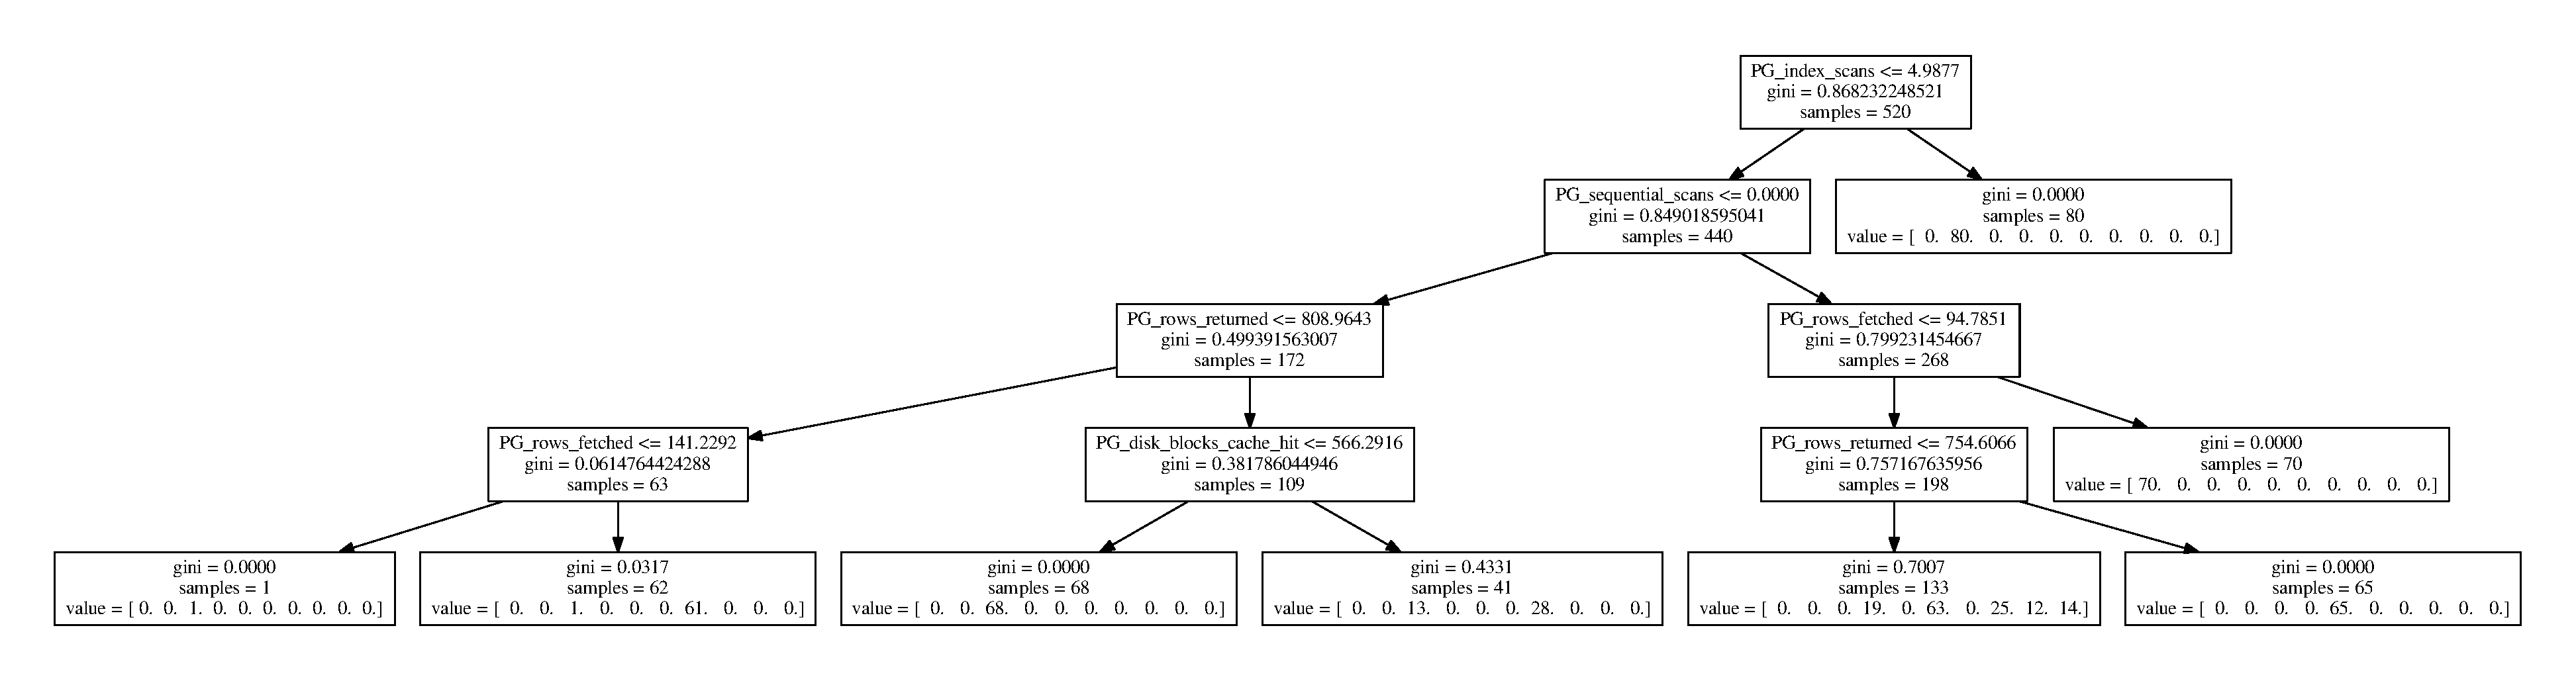
\includegraphics[width=\linewidth]{figure/tree_4.pdf}}
    \caption{Decision tree with max depth set to 4.}
    \label{fig:tree_4}
\end{figure*}

\begin{figure}[h!]
    \centering
	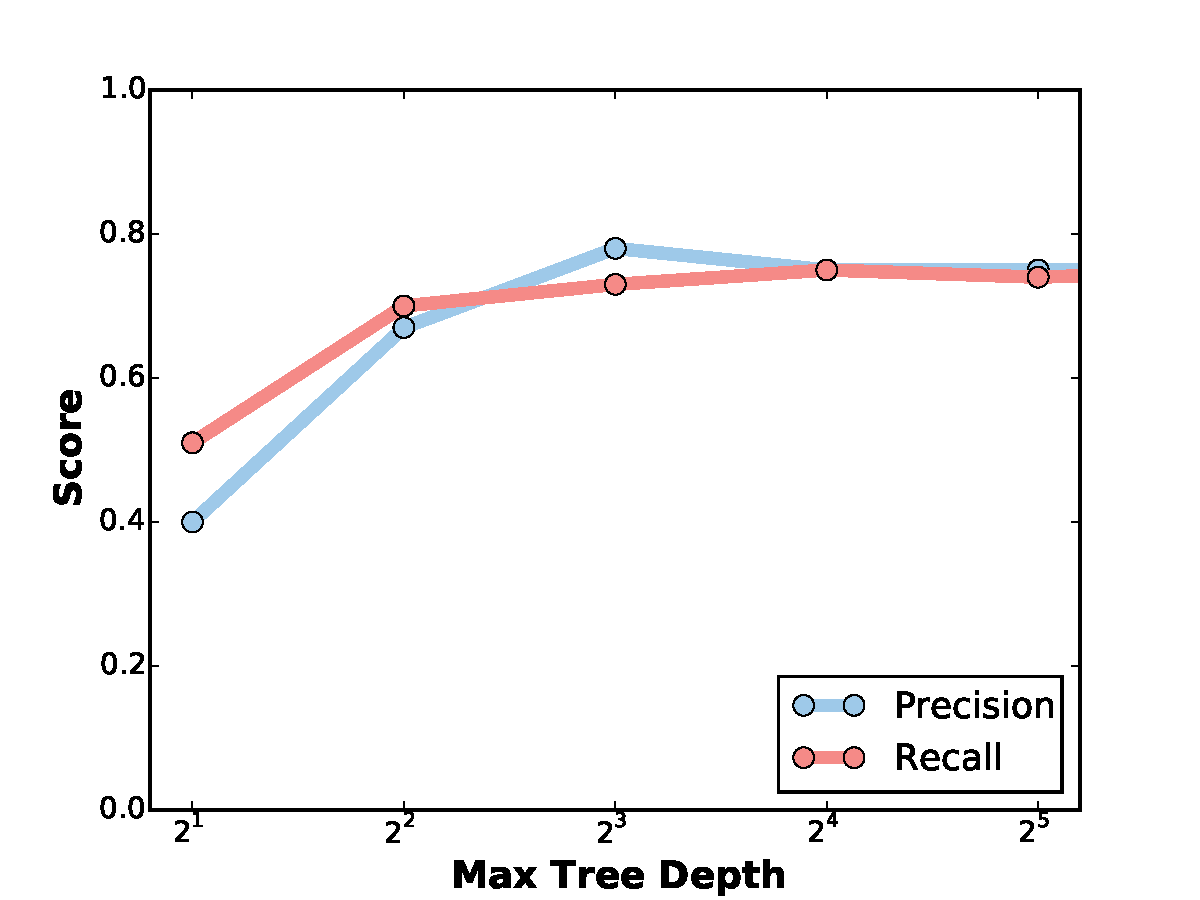
\includegraphics[width=0.7\linewidth]{figure/depth.pdf}
	\caption{Impact of max depth on the accuracy of the decision tree.}
\end{figure}

\begin{figure}[h!]
    \centering
	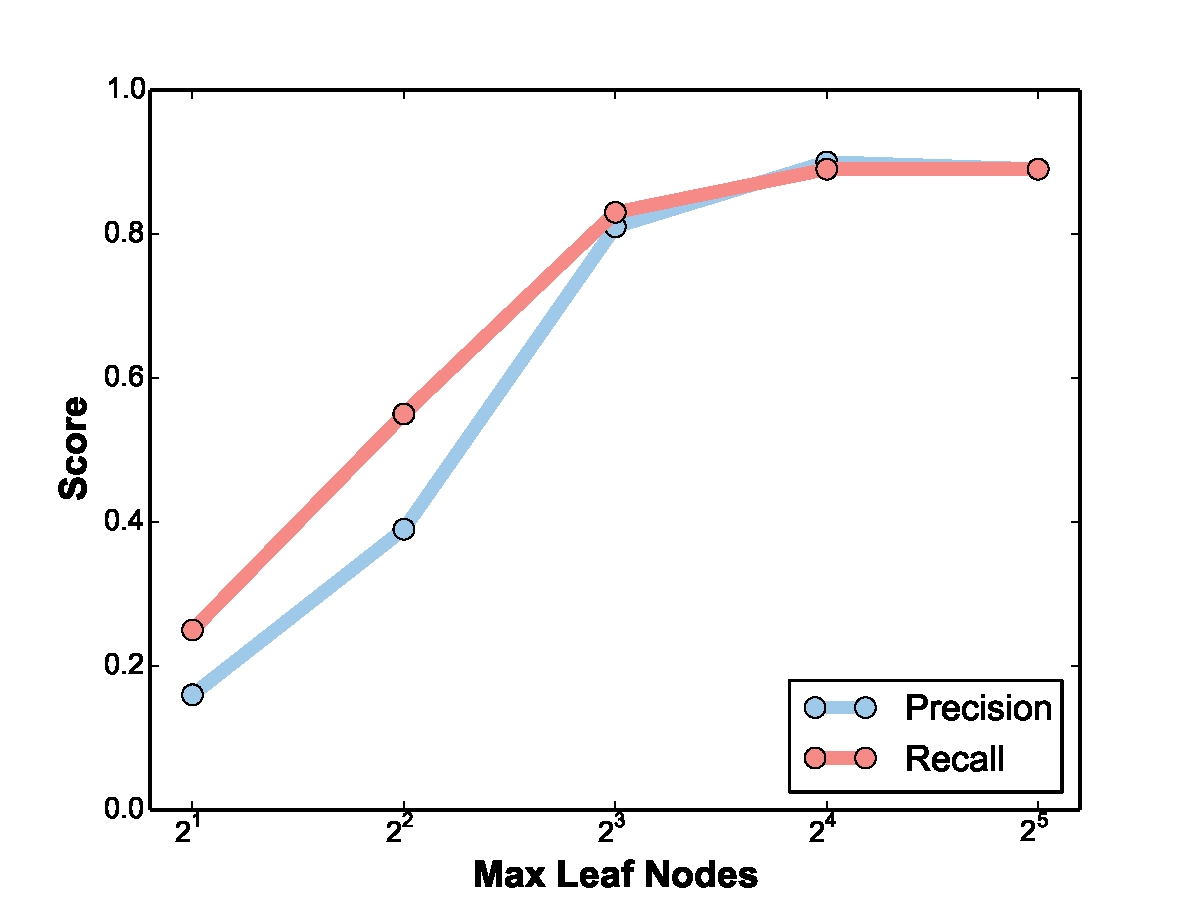
\includegraphics[width=0.7\linewidth]{figure/leaves.pdf}
	\caption{Impact of max leaf nodes on the accuracy of the decision tree.}
\end{figure}

\begin{table}[h!]
\centering
\small{
  \centering
  \begin{tabular}{l|llll} 
	\toprule
   		Class &  Precision  &  Recall &  F1-score  &  Support  \\    
    \midrule
		0.0   &    1.00   &   0.00   &   1.00   &     84   \\
        1.0   &    0.99   &   1.00   &   0.99   &     74   \\
        2.0   &    0.98   &   0.99   &   0.98   &     81   \\
        3.0   &    0.54   &   0.39   &   0.45   &     18   \\
        4.0   &    1.00   &   1.00   &   1.00   &     69   \\
        5.0   &    1.00   &   0.99   &   0.99   &     70   \\
        6.0   &    1.00   &   0.95   &   0.97   &     60   \\
        7.0   &    0.41   &   0.95   &   0.57   &     19   \\
        8.0   &    0.00   &   0.00   &   0.00   &     17   \\
        9.0   &    0.56   &   0.52   &   0.54   &     27   \\
    \midrule
Avg / Total   &    0.90   &   0.91   &   0.90   &    519   \\
   \bottomrule
   \end{tabular}
 }
%\nocaptionrule
\caption{Per-class accuracy of the default decision tree.}
\label{tab:dt_stats}
\end{table}



